
% $Header: /cvsroot/latex-beamer/latex-beamer/solutions/generic-talks/generic-ornate-15min-45min.en.tex,v 1.5 2007/01/28 20:48:23 tantau Exp $

\documentclass[smaller]{beamer}
\mode<presentation>
{
  \usetheme{Singapore}
  \usefonttheme[onlymath]{serif}
  % or ...
 %  \setbeamercovered{transparent}
  % or whatever (possibly just delete it)
}


\usepackage[czech]{babel}
% or whatever
\usepackage[utf8]{inputenc}
% or whatever
%\usepackage{times}
%\usepackage[T1]{fontenc}
% Or whatever. Note that the encoding and the font should match. If T1
% does not look nice, try deleting the line with the fontenc.


\title{PAS01 - Exploratorní statistika}

\author{Jan B\v rezina}
\institute % (optional, but mostly needed)
{
  %\inst{2}%
  Technical University of Liberec
}


% If you wish to uncover everything in a step-wise fashion, uncomment
% the following command: 

%\beamerdefaultoverlayspecification{<+->}

% ***************************************** SYMBOLS
\def\div{{\rm div}}
\def\Lapl{\Delta}
\def\grad{\nabla}
\def\supp{{\rm supp}}
\def\dist{{\rm dist}}
%\def\chset{\mathbbm{1}}
\def\chset{1}

\def\Tr{{\rm Tr}}
\def\sgn{{\rm sgn}}
\def\to{\rightarrow}
\def\weakto{\rightharpoonup}
\def\imbed{\hookrightarrow}
\def\cimbed{\subset\subset}
\def\range{{\mathcal R}}
\def\leprox{\lesssim}
\def\argdot{{\hspace{0.18em}\cdot\hspace{0.18em}}}
\def\Distr{{\mathcal D}}
\def\calK{{\mathcal K}}
\def\FromTo{|\rightarrow}
\def\convol{\star}
\def\impl{\Rightarrow}
\DeclareMathOperator*{\esslim}{esslim}
\DeclareMathOperator*{\esssup}{ess\,sup}
\DeclareMathOperator{\ess}{ess}
\DeclareMathOperator{\osc}{osc}
\DeclareMathOperator{\curl}{curl}

%\def\Ess{{\rm ess}}
%\def\Exp{{\rm exp}}
%\def\Implies{\Longrightarrow}
%\def\Equiv{\Longleftrightarrow}
% ****************************************** GENERAL MATH NOTATION
\def\Real{{\rm\bf R}}
\def\Rd{{{\rm\bf R}^{\rm 3}}}
\def\RN{{{\rm\bf R}^N}}
\def\D{{\mathbb D}}
\def\Nnum{{\mathbb N}}
\def\Measures{{\mathcal M}}
\def\d{\,{\rm d}}               % differential
\def\sdodt{\genfrac{}{}{}{1}{\rm d}{{\rm d}t}}
\def\dodt{\genfrac{}{}{}{}{\rm d}{{\rm d}t}}

\def\vc#1{\mathbf{\boldsymbol{#1}}}     % vector
\def\tn#1{{\mathbb{#1}}}    % tensor
\def\abs#1{\lvert#1\rvert}
\def\Abs#1{\bigl\lvert#1\bigr\rvert}
\def\bigabs#1{\bigl\lvert#1\bigr\rvert}
\def\Bigabs#1{\Big\lvert#1\Big\rvert}
\def\ABS#1{\left\lvert#1\right\rvert}
\def\norm#1{\bigl\Vert#1\bigr\Vert} %norm
\def\close#1{\overline{#1}}
\def\inter#1{#1^\circ}
\def\ol#1{\overline{#1}}
\def\ul#1{\underline{#1}}
\def\eqdef{\mathrel{\mathop:}=}     % defining equivalence
\def\where{\,|\,}                    % "where" separator in set's defs
\def\timeD#1{\dot{\overline{{#1}}}}

% ******************************************* USEFULL MACROS
\def\RomanEnum{\renewcommand{\labelenumi}{\rm (\roman{enumi})}}   % enumerate by roman numbers
\def\rf#1{(\ref{#1})}                                             % ref. shortcut
\def\prtl{\partial}                                        % partial deriv.
\def\Names#1{{\scshape #1}}
\def\rem#1{{\parskip=0cm\par!! {\sl\small #1} !!}}

\def\Xint#1{\mathchoice
{\XXint\displaystyle\textstyle{#1}}%
{\XXint\textstyle\scriptstyle{#1}}%
{\XXint\scriptstyle\scriptscriptstyle{#1}}%
{\XXint\scriptscriptstyle\scriptscriptstyle{#1}}%
\!\int}
\def\XXint#1#2#3{{\setbox0=\hbox{$#1{#2#3}{\int}$}
\vcenter{\hbox{$#2#3$}}\kern-.5\wd0}}
\def\ddashint{\Xint=}
\def\dashint{\Xint-}

% ******************************************* DOCUMENT NOTATIONS
% document specific
\def\rh{\varrho}
\def\vl{{\vc{u}}}
\def\th{\vartheta}
\def\vx{\vc{x}}
\def\vX{\vc{X}}
\def\vr{\vc{r}}
\def\veta{\vc{\eta}}
\def\dx{\,\d\vx}
\def\dt{\,\d t}
\def\bulk{\zeta}
\def\cS{\close{S}}
\def\eps{\varepsilon}
\def\phi{\varphi}
\def\Bog{{\mathcal B}}
\def\Riesz{{\mathcal R}}
\def\distr{\mathcal D}
\def\Item{$\bullet$}

\def\MEtst{\mathcal T}
%***************************************************************************
\setbeamercolor{my blue}{fg=blue}
\def\blue#1{{\usebeamercolor[fg]{my blue} #1}}
\setbeamercolor{my green}{fg=green}
\def\green#1{{\usebeamercolor[fg]{my green} #1}}
\setbeamercolor{my red}{fg=red}
\def\red#1{{\usebeamercolor[fg]{my red} #1}}
\def\xskip{{\vspace{2ex}}}

\begin{document}

\begin{frame}
  \titlepage
\end{frame}

% zvýraznění definovaného pojmu
\def\df{\usebeamercolor[fg]{my red}\it}
\begin{frame}{Příklad: spokojenost s menzou}
Chcete získat věrohodné informace o spokojenosti strávníků v menze.\\ 
Co uděláte? 

\pause
\begin{enumerate}
\item Koho se ptáme? \\
      \pause (úplné vs. výběrové šetření)\\
      \pause otázka věrohodnosti 
      
\item Na co se ptáme? \\
      \pause (druhy proměnných - veličin, které přiřazujeme prvkům populace)
\end{enumerate}

// Kniha od Kamila Nesetrial a prislusna data:
http://www.statistik.tuwien.ac.at/StatDA/R-scripts/
http://www.statistik.tuwien.ac.at/StatDA/DASplusR/

\end{frame}


\begin{frame}{Populace a výběry}
\blue{Populace} - množina objektů, o kterých chceme něco zjistit 
\begin{description}
\item[konečná] - občané ČR, všichni strávníci menzy, resp. jejich návštěvy
\item[nekonečná] - hustota hvězd na obloze, existuje nekonečno podmnožin - všechny možné polohy dalekohledu\\
  - rozbor vody, opět nekonečno podmnožin - všechny 1ml vzorky z vody protekající daným místem během roku\\
  Brát za populaci oblohu, nebo všechny podmnožiny oblohy?
\end{description}

\blue{Výběrové šetření} - uvažujeme konečný počet prvků (konečné) populace resp. konečný počet podmnožin (nekonečné) populace;
                          snažíme se o \blue{náhodný výběr}, tj. každý možný výběr je stejně pravděpodobný
                          

Výhody:
\begin{itemize}
\item ekonomické zvláště u rozsáhlých populací
\item výsledky i v případě nedostupnosti celé populace
\item možnost destruktivního testování
\end{itemize}
Nevýhody:
\begin{itemize}
\item Jak zajistit náhodnost výberu? (internetové průzkumy)
\item Pracnější analýza spolehlivosti výsledku
\end{itemize}
\end{frame}

\begin{frame}{Sledované proměnné}
\begin{itemize}
\item kvalitativní\\
	nominální (netříditelné) vs. ordinální (tříditelné)\\
	alternativní (poze dvě varianty) vs. množné (více variant)\\
\item kvantitativní \\
      \begin{itemize}
       \item diskrétní 
         \begin{itemize}
         \item konečná
         \item spočetná
         \end{itemize}
       \item spojitá
       \end{itemize}
\end{itemize}

Kvalitativní většinou zdánlivě převádíme na diskrétní proměnné (očíslování variant), ale nelze s nimi zacházet stejně.
\end{frame}

\section{Statistické charakteristiky kvalitativních proměnných}

\begin{frame}{Nominální proměnná}
\pause (výběrové) četnosti $n_i$ různých variant, $\sum n_i = n$ \\
       (výběrové) relativní četnosti $p_i=n_i/n$, $\sum p_i = 1$ \\
\pause  modus - varinata s nejvyšší četností       

\xskip

grafy: histogram, výsečový graf; !! uvádět absolutní četnosti, nebo rozsah výběru
\end{frame}       

\begin{frame}{Ordinální proměnná}
setříděné varianty: $x_1 < x_2 < \dots < x_n$\\
kumulativní četnost: $m_i = \sum_{j=1}^i n_i$\\
relativní kumulativní četnost: $F_i = \sum_{j=1}^i p_i = m_i / n$
\end{frame}

\begin{frame}{Grafy}
polygon kumulativních četností (čárový graf),\\
Paretův graf (i pro nominální uspořádaní sestupně podle četností) = polygon + histogram
\xskip

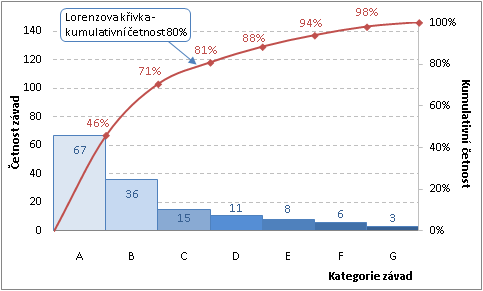
\includegraphics[scale=0.5]{graf-paretova-analyza.png} 
\end{frame}

\section{Statistické charakteristiky kvantitativních proměnných}
\begin{frame}{Charakteristiky pro kvantitativní proměnné}
\blue{míry polohy} : průměr, modus, kvantily (medián)[mo6nosti aprozximace kvantilů], minumum, maximum
\blue{míry rozptylu} : rozptyl, směrodatná odchylka, interkvartilové rozpětí, MAD
\blue{empirická distribuční funkce}
\end{frame}

\begin{frame}{Identifikace odlehlých pozorování}
\begin{enumerate}
\item kvartily + IQR
\item z- souřadnice
\item mediánová souřadnice
\end{enumerate}
\end{frame}

\begin{frame}{Výběrová šikmost a špičatost}
\blue{šikmost}:
\[
\alpha = \frac{n}{(n-1)(n-2)}\frac{\sum_{i=1}^{n} (x_i - \overline{x})^3}{s^3}
\]
\blue{špičatost}
\[
\beta = \frac{n(n+1)}{(n-1)(n-2)(n-3)}\frac{\sum_{i=1}{n} (x_i-\overline{x})^4}{s^4} - \frac{3(n-1)^2}{(n-2)(n-3)}
\]
\end{frame}

\begin{frame}{Krabicové grafy}
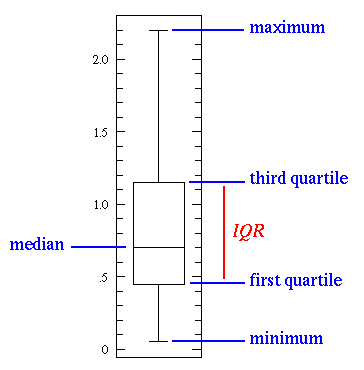
\includegraphics[scale=0.5]{simple_box_defs.png} 
\end{frame}

\begin{frame}{Třídění spojitých dat}
převod spojitých dat na diskrétní,\\
použití: histogram, statistické metody pro diskrétní veličiny
\begin{enumerate}
\item stejné šířky tříd: 
\item počet  $k = 1+\log_2 n=1+3.3 \log_10 n$
\item šířka $h = 2\ (IQR)\ n^{-1/3}$
\end{enumerate}
\end{frame}

\begin{frame}{Orientační charakteristiky normálního rozdělení}
\begin{itemize}
\item unimodální
\item nulová šikmost a špičatost
\item symetrie krabicového grafu
\item tvar třídního histogramu
\end{itemize}
\end{frame}

\end{document}


